\documentclass{article}
\usepackage{graphicx} % Required for inserting images
\usepackage{amsmath,amssymb,amsfonts}
\usepackage{algorithmic}
\usepackage{textcomp}
\usepackage{float}
\usepackage{etoolbox}
\usepackage{hyperref}
\usepackage{hyperref}
\usepackage{tikz}
\usepackage{fontawesome}
\usepackage{caption}
\usepackage{url}
\usepackage{listings}
\usepackage{pdfpages}
\usepackage[english]{babel}
\usepackage{scalerel}
\usepackage{xcolor,colortbl}
\usepackage[linesnumbered,ruled,vlined]{algorithm2e}
\usepackage{amsmath}
\usepackage{amssymb}
\usepackage{multirow}

\title{A Voter-to-Voter Internet Voting Protocol}
\author{Stanislaw Baranski}
\date{December 2023}

\begin{document}

\maketitle


\section{Introduction}
Voting is one of the most popular mechanisms for collective decision-making, prevalent in all types of communities including: non-government organizations, boardrooms, housing associations, regional contests and plebiscites, domestic presidential elections, as well as all forms of global voting that take place on the internet.

The act of vote can occur in different ways including paper-based precinct voting, mail-in ballots, electronically using direct-recording electronic (DRE) voting machine, and internet voting~\cite{parkGoingBadWorse2021}.

As proposed by Vitalik Buterin\cite{buterinBlockchainVotingOverrated2021} each voting (or more broadly, each collective decision-making) method faces a trilemma allowing it to choose only two out of three properties:

\begin{itemize}
    \item \textbf{Democratic}, means that the method ensures easy and equal (egalitarian) decision input for all eligible voters;
    \item \textbf{Secure}, means that the voting is confident, fair, transparent, private, and resistant to attack vectors;
    \item \textbf{Efficient}, means that the method is easy, fast, and cheap.
\end{itemize}

In traditional political elections, security and democracy are essential factors, thus efficiency is sacrificed. Social media votings are democratic and efficient, thus security is sacrificed. An example of an efficient and secure collective decision-making mechanism is the market, where users express their preferences by purchases, increasing the lobbying power of such a company. Markets, however, are not democratic, making them a poor fit for decisions regarding public goods. 

The inefficiency of traditional voting makes them costly and thus limits their frequency usually to a single vote once every one to six years~\cite{buterinBlockchainVotingOverrated2021}.

Voting over the internet (i-voting) seems to be an ideal solution especially when online banking is so prevalent nowadays. Arguably, internet voting is the most conventional, cheapest, fastest, and safest (e.g., during the outbreak of COVID-19), and hence, a preferred method for conducting voting.

Internet voting can increase turnout and the frequency of votings, but most importantly, it can catalyze the further development of modern democracy. Enabling practical applications of direct democracy, liquid democracy, and all other sorts of voting methods like Quadratic Voting, Approval voting, Alternative vote, Score voting, and many others \cite{laslierLoserPluralityVoting2011}.

Moreover, visions of smart cities, crypto cities \cite{buterinCryptoCities2021}, Decentralised Autonomous Organisations (DAO)~\cite{wangDecentralizedAutonomousOrganizations2019}, and other forms of algorithmic governance~\cite{GovernmentAlgorithm2022} rely heavily on the existence of electronic voting, so there is a high need for such systems, as they would enable further development of modern democracy.

Undoubtedly, there is a high demand for internet voting protocol. However, except a minor cases like Switzerland and Estonia, the progress of introducing modern democracy tools is still slow comparing to e.g., online banking.

Internet voting has been researched for many years, especially in domains such as cryptography, which is an inevitable part of system security. Many of them doubt the possibility of conducting public voting over the internet \cite{parkGoingBadWorse2021, mearianWhyBlockchainbasedVoting2019, shanklandNoBlockchainIsn2018, leeBlockchainbasedElectionsWould2018, schneierBlockchainVoting2020, schneierBlockchainTrust2019}. The resistance lies—among others—in insufficient confidence in the technology and a need for trust in the authorities controlling the voting process.

The criticism against internet voting comes down to two arguments:

\begin{enumerate}
    \item No software is flawless, therefore it can not be trusted.
    \item There is too strong a trust assumption in authorities controlling the voting process.
\end{enumerate}

A recent paper from MIT researchers~\cite{parkGoingBadWorse2021} argues that any paperless voting is a bad design. High-quality software (at the 90th percentile for the software industry) contains on average one defect in every ten thousand lines of code~\cite{llaguno2017CoverityScan2017}. Some errors lead to malfunctioning, and some are "exploitable vulnerabilities", which allow an adversary to take control over the computer and install fraudulent software.

The argument is that an undetected change or error in a system's software should not cause an undetectable change in the election outcome, and since every software is flawed, there is no such guarantee.

However, recent advances in cryptography can guarantee correct program execution using zero-knowledge proofs~\cite{parnoPinocchioNearlyPractical2013}. Using such a publicly available proving system, anyone can verify the correctness of the voting process. Because the proofs of correctness are just cryptographic materials, everyone can write their implementation of a verifier program, achieving the software independence requirement stated by the authors of~\cite{parkGoingBadWorse2021}.

Even if the software can be trusted, another argument is that the hardware (voters' devices) can not be trusted. They argue that "internet voting protocols' security relies upon voters' devices being uncompromised and functioning as intended, an unrealistic assumption~\cite{parkGoingBadWorse2021}.

Although hardware (even the Trusted Hardware~\cite{sionTrustedHardware2009} like Intel® Software Guard Extensions~\cite{mckeenIntelSoftwareGuard2016}) keeps getting broken~\cite{goodinIntelSGXVulnerable2020, IntelSGXBroken2019, bulckForeshadowExtractingKeys}, there is a constant improvement in the security of the hardware. Especially, smartphones are being equipped with a secure area on their main processors called Trusted Execution Environment (TEE). For example, Apple's Secure Enclaves~\cite{SecureEnclave}, Samsung's Knox~\cite{kanonovSecureContainersAndroid2016}, HTC's Zion~\cite{exodusZION}, and ARM's TrustZone~\cite{ARMSecurityTechnology}. Generally, it is believed that cybersecurity is getting better, not worst~\cite{golombBelieveItCybersecurity2018}.

Moreover, the authors of~\cite{appelEvidenceBasedElectionsCreate2019} claim that "there is no perfect, infallible way to count votes. All methods including optical scan, touchscreen, and hand counting—are subject to errors, procedural lapses, and deliberate manipulation." Therefore, the argument is not about security or lack of it, but how much secure it is, and what are the trust assumptions.

The second biggest critique against internet voting is the required trust in authorities controlling the voting process. Concretely, the servers act like a pooling station where voters cast their votes. While in the real world the pooling station is located in a neutral place and the whole process is transparent to all voters, the digital pooling stations — servers — do not offer this evidence-based trust property~\cite{starkEvidenceBasedElections2012}.

According to the principle of the evidence-based election ~\cite{starkEvidenceBasedElections2012}, authorities that control the voting "should not only find the true winner but also provide the electorate convincing evidence that they did"~\cite{appelEvidenceBasedElectionsCreate2019}. Convincing evidence, according to the authors of~\cite{starkEvidenceBasedElections2012}, is achieved when the voting is both auditable and audited. The process is auditable when it provides a trustworthy audit trail that can ensure voting accuracy. The voting is audited when the electoral executed the trustworthy audit trail as a routine of casting a vote.

\textbf{Ideally, the whole voting process should be completely trustless, meaning that, there should be no trust assumptions other than in our perception.}

In practice, we rarely monitor the whole process of elections. Rather, we delegate that duty to staff responsible for conducting voting. We believe that at least one person is an honest observer who will alarm if something goes wrong.

So the evidence-based election~\cite{appelEvidenceBasedElectionsCreate2019}, in practice uses $1 \textrm{ of } N$ trust model~\cite{buterinTrustModels2020}, which means that the system is trusted as long as at least one person out of $N$ observers is honest, and in case of a fraud will reveal it.

However, if at some point, the group of observers drops to a few people, the chance of finding at least one honest observer reduces, and with it the trustworthiness of the whole election. Therefore, a voting process should involve a large number of observers — the larger the $N$, the more trusted the setup is.

The critique against internet voting system run by centralised authorities is that it requires the strongest assumption on $1\textrm{ of }1$ trust model as there is no way to provide the electorate convincing evidence that the running software is correct. This means that there is a single point of failure, an authority, which if compromised, breaks the trust.

There are two counterarguments to that critique. 
\begin{enumerate}
    \item First, even if the organizers are not trusted, by enforcing them to produce the cryptographic proof of tallying, they can not produce incorrect results as this incident would come to light during the proof verification.
    \item  The second is that the traditional centralized authority can be decentralised with the usage of distributed systems and consensus mechanisms, changing the trust model from $1 \textrm{ of } 1$ to either $N \textrm{ of } N$ where all actors have to work as expected, or $Few \textrm{ of } N$ where a few fixed set of nodes has to work correctly, or $\frac{N}{2} \textrm{ of } N$ where the system works correctly as long as the majority of nodes are working correctly. 
\end{enumerate}

When the trust assumption is violated some of the properties of the system fail. Depending on the system, the properties are liveness failure, or safety failure. Other times it's censorship-resistance, privacy, and/or correctness.

A particularly successful technology for decentralising trust is blockchain which natively guarantees immutability, verifiability, integrity, and censorship resistance. And hence blockchain become a popular platform for building trust-minimising platforms such as internet-voting protocols.

Even if Blockchain is not used, and instead distributed set of authorities (called Guardians) are running the voting system like Helios~\cite{adidaHeliosWebbasedOpenAudit2008} or ElectionGuard~\cite{ElectionGuard}. The burden of involving an external organiser still exists.

In this paper we propose an alternative architecture which generalises the trust model and allows to freely chose who becomes the trustee in the system. 

Figure ~\ref{fig:trust-models} presents the shift from internet votings based on trusted third party, to internet votings based on distributed third parties, to voter-to-voter protocols, and finally more realistic model delegated voter-to-voter protocol which we will discuss in this paper.

\begin{figure}
    \centering
    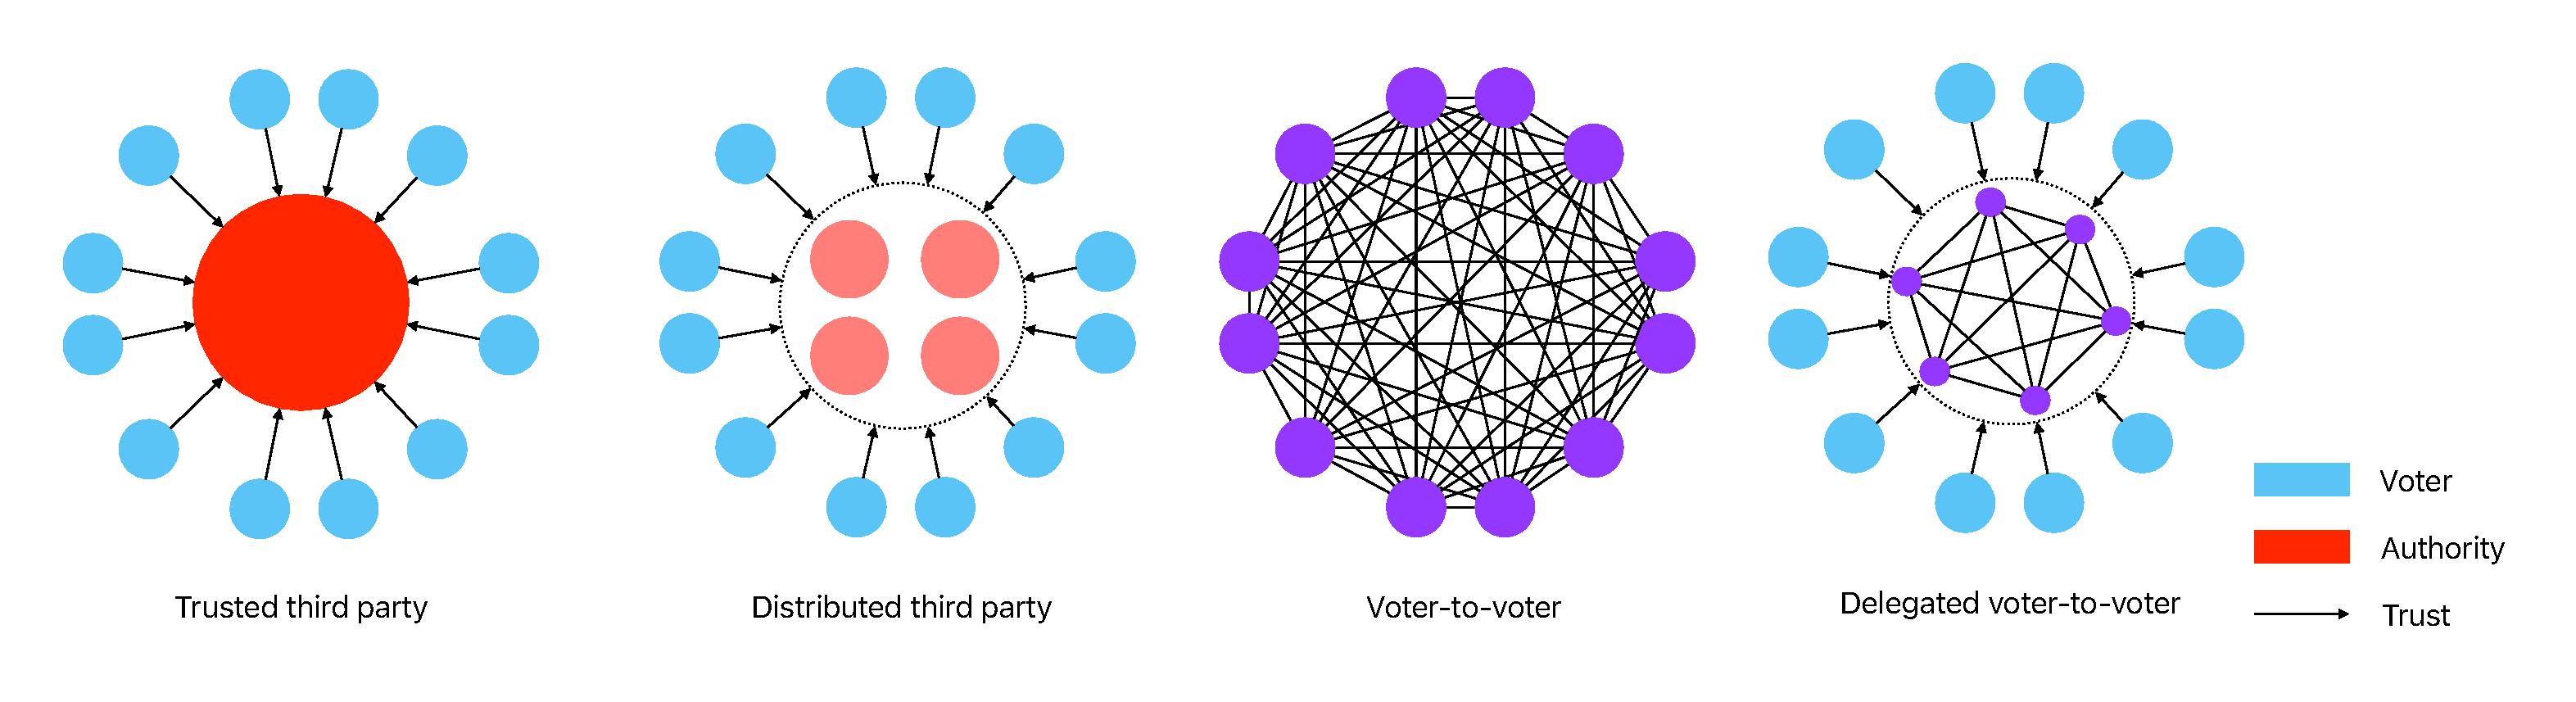
\includegraphics[width=\textwidth]{trust-models-voting.pdf}
    \caption{Four trust models: trusted third party, distributed authorities, peer-to-peer, delegated voter-to-voter}
    \label{fig:trust-models}
\end{figure}

The paper contributes to the state of the art in the following ways:
\begin{enumerate}
    \item We propose a novel technique for dynamic Distributed Key Generation (DKG) called Federated DKG (FDKG), which maps the structure of trust between the members of a group that wants to make an election. The technique works in a similar way to the Federated Byzantine Agreement (FBA) in the Stellar Consensus Protocol~\cite{mazieresStellarConsensusProtocol2015}.
    \item Based on the assumption that the majority of the most important members of the grouping will participate in all phases of voting (1. FDKG and 3. Tally) our protocol requires only one message (You-only-speak-once~\cite{gentryYOSOYouOnly2021}) to be sent by each participant which increases the practicality of our protocol.
    \item The protocol is robust to Byzantine nodes through the use of zero-knowledge proofs (zkSNARKs)~\cite{parnoPinocchioNearlyPractical2013}. Each message must have a proof of adherence to the rules of the algorithm.
    \item The privacy of the system is based on the honest majority assumption. The protocol achieves privacy as long as the majority of the most important nodes in the network are honest and do not collude.
    \item The system is robust against a subset of unavailable nodes (faulty nodes). Using threshold cryptography, the system allows a subset of nodes to decrypt the voting results so that no single node in the network is able to block the voting.
    \item The system is free of charge for the end user. The application is completely peer-to-peer thus avoiding any fees associated with transactions (as is the case with systems based on public blockchains) and the maintenance of a central coordinator (in the case of a private network or server).
\end{enumerate}

\section{Related work}
Most Internet protocols rely on a trusted third party. They differ in what the server can or cannot do. The honesty of the trusted third party determines either anonymity, privacy or coercion resistance properties.

Most of the current reserach on internet voting protocols uses some kind of blockchain for integral and transparent storage. 
Voatz~\cite{mooreWestVirginiaMobile2019}, 
Polys~\cite{PolysOnlineVoting}, 
OpenVoteNetwork~\cite{haoAnonymousVotingTworound2010}, MACI~\cite{ethereumfoundationMinimalAntiCollusionInfrastructure2022}.

However some projects achieve similar properties without using blockchain. Projects like Civitas, Swisspost/Scytl, iVoting, or ElectionGuard use some kind of distributed authorities to run the voting process. The trust model usually is $N \textrm{ of } N$ where all authorities have to work as expected. All the computation is done using some kind of Multi-Party Computation (MPC) protocol~\cite{boweMultipartyProtocolConstructing2018}.
These systems are not fully decentralised as they are based on a closed set of trusted entities called Guardians. In practice they are "Election Officials, Trustees Canvass Board Members, Government Officials or other trusted authorities who are responsible and accountable for conducting the election"~\cite{ElectionGuardWhoGuardian}.


Solutions built on public blockchains require voters to pay transaction fees.

Solutions built on private blockchains still need to be hosted somewhere, which costs money or creates a high entry point for non-technical people.

Compared to other public-blockchain-based solutions, our solution is free, which is arguably a big deal—paying for a vote must reduce the turnout.

Compared to private-blockchain-based solutions or ElectionGuard-like systems, in our system, there is no need to run the software on any centralised server(s), which is also arguably a big deal, especially in the case of small, informal voting. Someone has to run this server. For larger organisations like universities, it's not a problem as an IT department is responsible for hosting it. But for small organizations, it can be a problem. For example, Student Council Elections, Corporate Board Decisions, Homeowners Association Voting, NGOs, Town Hall Meetings, Union Voting, Talent Competitions, Open-source Projects, Start-up teams, Student communities, or Boardrooms. Running the software in a SaaS model, brings us back to the question of "who runs the message board and tallying software and can we trust them?" or even "who pays for it?".

In our solution, voters are running the software, so the question of "who runs the message board and tallying software and can we trust them?" changes to “do we trust that the majority (more concretely m-of-n voters) are honest?” Moreover, as the network is private p2p there is no problem of "who pays for it?". And because it's a private blockchain there are no transaction fees.

Below is a comparison table.

\newcommand{\fullmoon}{\tikz\filldraw[fill=black] (0,0) circle (0.5em);}
\newcommand{\newmoon}{\tikz\draw (0,0) circle (0.5em);}
\newcommand{\rightmoon}{\tikz\draw (0,0) circle (0.5em); \filldraw[fill=black] (0,0) arc (90:270:0.5em) -- cycle;}
\newcommand{\leftmoon}{\tikz\draw (0,0) circle (0.5em); \filldraw[fill=black] (0,0) arc (270:90:0.5em) -- cycle;}
\newcommand{\halfmoon}{\tikz\draw (0,0) circle (0.5em); \filldraw[fill=black] (0,-0.5em) rectangle (0,0.5em);}


\begin{table*}[!h]
\centering
\newcommand{\YES}{\cellcolor{red!50}Yes}
\newcommand{\NO}{\cellcolor{green!50}No}
\caption{A comparative analysis of three types of internet voting systems: Public Blockchain-based, Private Infrastructure-based, and Voter-to-Voter Network-based, highlighting their differences in transaction fees, service costs, user-friendliness, and trust dynamics.}
\begin{tabular}{p{0.2\textwidth}p{0.2\textwidth}p{0.17\textwidth}p{0.17\textwidth}p{0.21\textwidth}}
\noalign{\smallskip}\hline\noalign{\smallskip}
\textbf{Property} & \textbf{Centralised server} & \textbf{Private network} & \textbf{Public blockchain} & \textbf{Voter-to-Voter network}\\
\noalign{\smallskip}\hline\noalign{\smallskip}
Transaction fees & \NO & \NO & \YES & \NO \\
\hline
Service costs\footnote{The cost of service includes all costs related to implementation, maintenance, and fees} & \cellcolor{yellow!50} Medium & \cellcolor{red!50} High & \cellcolor{green!50} No  & \cellcolor{green!50} No \\
\hline
User-Friendliness & \cellcolor{green!50} High & \cellcolor{green!50}High & \cellcolor{red!50} Low & \cellcolor{yellow!50} Medium \\
\hline
Trust to\footnote{Trust is a broad term that refers to different properties of the system, but most of the time it answers the question of who holds the properties of censorship-resistance, privacy, and/or correctness.} & \cellcolor{red!50} Central authority & \cellcolor{yellow!50} Authorities\footnote{Examples of authorities are: "Election Officials, Trustees Canvass Board Members, Government Officials or other trusted authorities who are responsible and accountable for conducting the election", \href{http://www.electionguard.vote/basics/steps/1_Key_Ceremony/}{source}.} & \cellcolor{yellow!50} Miners & \cellcolor{yellow!50} Voters  \\
\noalign{\smallskip}\hline

\hline
\end{tabular}
\end{table*}

\section{System Architecture}
Designig a user application that is intended to work in peer-to-peer model is a complex task. The main challenge is to overcome the networking problems, weak availability and limited resources of end-devices such as smartphones and laptops.

\paragraph{Objectives}
In designing the architecture of the protocol, we were guided by several key objectives, aimed at addressing the fundamental challenges and requirements of an secure and practical internet voting system. These objectives are:

\begin{enumerate}
    \item \textbf{Privacy}: Ensuring voter privacy under the honest-majority assumption, safeguarding vote confidentiality.
    \item \textbf{Distributed Architecture}: Eliminating central authority to enhance system resilience and reduce single points of failure.
    \item \textbf{Robustness}: Designing for ease of use and practicality, ensuring high availability and preventing nodes from blocking the voting process.
    \item \textbf{Lightweight Implementation}: Facilitating operation on common devices like laptops and smartphones to ensure accessibility and scalability.
    \item \textbf{Zero-Fee Participation}: Ensuring that voting is free of charge to increase turnout and support democratic engagement.
\end{enumerate}

\subsection{Achieving System Objectives}
Each objective in the Voter-to-Voter Internet Voting Protocol is meticulously addressed to ensure the system's effectiveness and alignment with democratic principles:

\paragraph{Privacy}
The protocol ensures voter privacy through advanced cryptographic techniques, primarily operating under the honest-majority assumption. TODO

\paragraph{Distributed Architecture}
To eliminate reliance on a central authority, the protocol is built on a distributed network of nodes.. TODO

\paragraph{Robustness}
The system is designed for practicality and ease of use, ensuring that it is accessible to a wide range of users.. TODO

\paragraph{Lightweight Implementation}
By optimizing the system for lightweight operation, it can be executed on commonly available devices such as laptops and smartphones. TODO

\paragraph{Zero-Fee Participation}
Zero-fee participation is ensured through the use of a peer-to-peer ad-hoc network. TODO

\paragraph{Ad-hoc Blockchain Network and Networking}
The foundation of the system is an ad-hoc blockchain network.


% Party
\newcommand{\PartySecretKey}[1]{\ensuremath{s_{#1}}}
\newcommand{\Party}[1]{\ensuremath{P_{#1}}}

% Voting keys
\newcommand{\EncryptionKey}{\textbf{E}}
\newcommand{\DecryptionKey}{\textbf{d}}

% Partial voting keys
\newcommand{\PartialDecryptionKey}[1]{\ensuremath{d_{#1}}}
\newcommand{\PartialEncryptionKey}[1]{\ensuremath{E_{#1}}}

% Ciphertexts
\newcommand{\EncryptedPartialDecryptionKeyShare}[2]{\ensuremath{C_{#1,#2}}}
\newcommand{\SetOfEncryptedPartialDecryptionKeys}{\ensuremath{\mathbb{C}}}
\newcommand{\SetOfFDKG}{\ensuremath{\mathbb{D}}}
\newcommand{\SetOfSharesOfPartialDecryption}{\ensuremath{\mathbb{C}}}

% Shares
\newcommand{\IthDecryptionKey}[1]{\ensuremath{d_{#1}}}
\newcommand{\IthEncryptionKey}[1]{E_{#1}}

% Private channel
\newcommand{\DecryptionUsingOf}[2]{\ensuremath{\texttt{Dec}_{#1}(#2)}}
\newcommand{\EncryptionUsingOf}[2]{\ensuremath{\texttt{Enc}_{#1}(#2)}}

\newcommand{\PartialDecryptionKeyShare}[2]{\ensuremath{[d_{#1}]_{#2}}}


\newcommand{\ProofFDKG}[1]{\ensuremath{\textrm{PROOF}_{#1,\textrm{FDKG}}}}

\newcommand{\ProofFDKGInformal}{"Given \PartialEncryptionKey{i}, \EncryptedPartialDecryptionKeyShare{i}{j} and $\Party{j} \in \GuardianSetOf{i}$, I know $f_i = a_0, \dots, a_{t-1}$, $r1_1,\dots,r1_k$, and $r2_1,\dots,r2_k$, s.t. $\PartialEncryptionKey{i}=a_0G$ and the \EncryptedPartialDecryptionKeyShare{i}{j} is an encrypted value of a polynomial $f_i(\cdot)$ applied to $j$"}

\newcommand{\ProofBALLOT}[1]{\ensuremath{\textrm{PROOF}_{#1,\textrm{BALLOT}}}}

\newcommand{\ProofBALLOTInformal}{"Given \EncryptionKey{} and \Ballot{i} = $(C1, C2)$, I know \BlindingFactor{i}, and \Vote{i} s.t. $\Vote{i} \in \{2^0, 2^j, \ldots, 2^{(l-1)j}\}$ and $\Ballot{i} = (\BlindingFactor{i} G,\ \BlindingFactor{i} \EncryptionKey{} + \Vote{i})$"}

\newcommand{\ProofPD}[1]{\ensuremath{\textrm{PROOF}_{#1,\textrm{PD}}}}

\newcommand{\ProofPDInformal}{"Given $\TotalA{}, \PartialDecryptionFrom{i}, \PartialEncryptionKey{i}$, I know a partial decryption key $\PartialDecryptionKey{i}$ s.t. $\PartialEncryptionKey{i} = \PartialDecryptionKey{i} \cdot G$ and $\PartialDecryptionFrom{i} = \PartialDecryptionKey{i} \cdot \TotalA{}$"}

\newcommand{\ProofPDS}[2]{\ensuremath{\textrm{PROOF}_{#1,#2,\textrm{[PD]}}}}

\newcommand{\ProofPDSInformal}{"Given $\SharePartialDecryptionFromTo{j}{i}, \EncryptedPartialDecryptionKeyShare{j}{i}, \TotalA$, I know a secret key $\PartySecretKey{i}$ s.t. $\SharePartialDecryptionFromTo{j}{i} = \TotalA \cdot \PartialDecryptionKeyShare{j}{i}$ where $\PartialDecryptionKeyShare{j}{i} = \DecryptionUsingOf{\PartySecretKey{i}}{\EncryptedPartialDecryptionKeyShare{j}{i}}$"}



\newcommand{\Ballot}[1]{\ensuremath{B_{#1}}}

\newcommand{\Generator}[1]{\ensuremath{H_{#1}}}
\newcommand{\BlindingFactor}[1]{\ensuremath{r_{i}}}
\newcommand{\Vote}[1]{\ensuremath{v_{#1}}}

\newcommand{\GuardianSetOf}[1]{\ensuremath{\mathbb{G}_{#1}}}
\newcommand{\TotalA}{\ensuremath{C1}}
\newcommand{\TotalB}{\ensuremath{C2}}
\newcommand{\BallotA}[1]{\ensuremath{C1_{#1}}}
\newcommand{\BallotB}[1]{\ensuremath{C2_{#1}}}

\newcommand{\G}{\ensuremath{G}}


% Partial Decryption Results
\newcommand{\SharePartialDecryptionFromTo}[2]{\ensuremath{[\mathrm{PD}_{#1}]_{#2}}}

\newcommand{\PartialDecryptionFrom}[1]{\ensuremath{\mathrm{PD}_{#1}}}

\section{Voting Protocol}
Our voting protocol is a combination of 3-round voting scheme proposed in~\cite{schoenmakersLectureNotesCryptographic2018}, multi-candidate encoding proposed in~\cite{haoAnonymousVotingTworound2010}, and Federated DKG that we propose in this paper. 

We use Threshold ElGamal Cryptosystem which guarantees the decryptiability even in case of unavailable guardians.

\paragraph*{Assumptions}
\begin{enumerate}
    \item All communication is done over a public Message board.
    \item Authenticated public channels are available for every participant, achieved by a public message board and digital signatures.
    \item Private channels are available for every participant, achieved by a public message board, and ElGamal public key encryption.
    \item Each participant \Party{i} consists of key pair (\PartySecretKey{i}, \Party{i}), where $\PartySecretKey{i} \in_{R} \mathbb{Z}_q$ is a randomly selected secret key, and $\Party{i} = \PartySecretKey{i} \cdot \G$ is the corresponding public-key. We use the same notation for a party and its public key, \Party{i}, as parties are identified by their public keys only.
    \item We use Elliptic Curve Cryptography, specifically \href{babyJubJub curve}{https://z.cash/technology/jubjub/}.
    \item Participation in the protocol is equivalent to agreeing to: \begin{enumerate}
        \item Elliptic Curve $E(\mathbb{Z}_q)$, with the base (generator) point on the curve $G$;
        \item Set of eligible voters (participants) $\vec{P}=\{P_1,\dots,P_n\}$, where $n$ is the number of all voters;
        \item Set of $l$ options $\vec{C}=\{C_1, \dots, C_l\}$, where $l$ is the number of all candidates. % TODO fix
    \end{enumerate}
    \item Public-key encryption is realised using ElGamal cryptosystem. $EG_{P}(\cdot)$ is the encryption algorithm for public key $P$, and $EG_{s}(\cdot)$ is the decryption algorithm using corresponding secret key $s$.
\end{enumerate}

\subsubsection{Private Channel}

Each user use a private authenticated channel to send encrypted messages to other parties. We follow the ElGamal encryption on the BabyJub curve scheme as described in~\cite{ElGamalEncryptionDecryption2020,jieWeijiekohElgamalbabyjub2023}.  In this encryption method, we start with a plaintext scalar $m$, which is an element in the BabyJub finite field. To encrypt this scalar, we first change it into a point on the BabyJub elliptic curve using a function \texttt{encodeToMessage}. This function samples a random value \( r \in_{R} \mathbb{Z}_q\), computes a point \( rG \), and subtracts the $m$ value from the x-coordinate of the point. As a result the ciphertext is a triple of two elliptic curve points and one field element $(C_1, C_2, \Delta=rG.x - m)$. See Algorithm~\ref{alg:encryption}.

The decryption of $(C_1, C_2, \Delta)$ involves standard ElGamal decryption and then adding x-delta $\Delta$ to the x-coordinate of the output point. See Algorithm~\ref{alg:decryption}.

\begin{algorithm}
    \SetAlgoNlRelativeSize{0}
    \SetAlgoNlRelativeSize{-1}
    \SetAlgoNlRelativeSize{1}
    \SetKwInOut{Input}{Input}
    \SetKwInOut{Output}{Output}
    \caption{$\texttt{Enc}_{P_i}$}
    \label{alg:encryption}
    
    \Input{A scalar $m$}
    \Output{A tripe $(C_1, C_2, \Delta)$}
    
    $k \gets_R \mathbb{Z}_q$\;
    $r \gets_R \mathbb{Z}_q$\;
    $C_1 = kG$\;
    $M = rG$\;
    $C_2 = kP + M$\;
    $\Delta = M.x - m$\;
    \Return $(C_1, C_2, \Delta)$
\end{algorithm}

\begin{algorithm}
    \SetAlgoNlRelativeSize{0}
    \SetAlgoNlRelativeSize{-1}
    \SetAlgoNlRelativeSize{1}
    \SetKwInOut{Input}{Input}
    \SetKwInOut{Output}{Output}
    \caption{$\texttt{Dec}_{s_i}$}
    \label{alg:decryption}
    
    \Input{A tripe $(C_1, C_2, \Delta)$}
    \Output{A scalar $m$}
    
    $M = C_2 - s_i C_1$\;
    $m = M.x - \Delta$\;
    \Return $m$
\end{algorithm}



\subsection{Federated Distributed Key Generation}
The goal of DKG protocol is to jointly generate the voting key-pair without any party learning the secret (decryption) key. Each party $P_1,\dots,P_n$ learns only its share of the secret (decryption) key, while public (encryption) key is publicly known. Moreover we want the threshold property, meaning that, not every party that participated in the key generation needs to participate in the tally phase.

\subsubsection*{Secret Sharing}

Threshold secret sharing can be done using Shamir Secret Sharing (SSS), which allows a dealer to encode secret key $s$ into a random polynomial $\mathbf{f}(X) = a_0 + a_1X + a_2X^2 + \dots + a_{t-1}X^{t-1}$, where $a_0,a_1,\dots,a_{t-1} \in_R \mathbb{F}_q$; the secret key $s=a_0=\mathbf{f}(0)$ and $t-1$ is the degree of polynomial. The shares are computed by evaluating function $\mathbf{f}(\cdot)$ at coordinates $(x=i,y=\mathbf{f}(i))$, $i \neq 0$. Following a Lagrange Theorem, $t$ number of points on the polynomial $\mathbf{f}(X)$ allows for reconstructing the polynomial and hence extract secret key by computing $s = \mathbf{f}(0)$.

\subsubsection*{Distributed Key Generation}
We don't want any party to become a dealer (and learn the secret value $s$), and so, we have to distribute the generation of polynomial $\mathbf{f}(X) \in_R \mathbb{Z}_q[X]$ across all parties $\vec{P}$. It is done by having each party pick a random polynomial $f_{i}(X) \in \mathbb{Z}_q[X]$, and then define the final polynomial \[\mathbf{f}(X)=\sum_{i=1}^{n}f_i(X)\] Hence, the voting secret (decryption) key $\mathbf{d}$ and voting public (encryption) key $\mathbf{E}$ are: $$\mathbf{d}=\mathbf{f}(0)$$ $$\mathbf{E}=\mathbf{d} \cdot \G$$ 

To prevent misbehaviour of parties (sending arbitrary values) we use a more sophisticated version of SS called Publicly Verifiable Secret Sharing (\href{PVSS}{https://www.win.tue.nl/~berry/papers/crypto99.pdf}), which involves zero-knowledge proofs attesting that the correct relation between values holds.


\subsubsection*{Dynamic Distributed Key Generation}
Distributed Key Generation in its original form requires known and fixed number of participants. It's because, underneath, it relies on SSS which uses polynomials of known degree $t$. The degree is fixed at the beginning of the protocol and can not be changed.

\textbf{We want the DKG phase to be optional}, so the total number of participants is unknown, and so the $t$ is also unknown. As a result, we need a scheme that allows for dynamic updating the number of participants and the threshold.

To our best knowledge, the scheme which allows for dynamic DKG~\cite{delerableeDynamicThresholdPublickey2008} requires all parties to be online for the duration of the DKG (possible a few hours). It's done by reconstructing the key by current participants and resharing it again with the new participant.

We believe it is an unpractical assumption. We want the protocol to be non-interactive, meaning that the party sends only one message and then can leave.

% consider this path of reasoning:
% - We want the DKG and Tally rounds to be optional
% - Threshold Encryption works on Shamir Secret Sharing (SSS)
% - SSS works on polynomials
% - Polynomials have to have a defined fixed degree $t$
% - We want the DKG phase to be optional, so the total number of participants is unknown, and so the $t$ is also unknown
% - Therefore, we can not define the polynomial of unknown size


\subsection{Round 1. Federated Distributed Key Generation}

We propose a novel technique for dynamic DKG that works similarly to \href{Stellar Consensus Protocol}{https://developers.stellar.org/docs/fundamentals-and-concepts/stellar-consensus-protocol}~\cite{mazieresStellarConsensusProtocol2015}.

Every party can (but does not have to) participate in the DKG phase. The actual number of parties that participate is denoted by $m$ where the maximum number is $n$. Since we focus on small scale votings where participants know each other, we make a social assumption, that each participant trusts $k$ other parties. Then we chose a threshold $t$ of parties, which allows for key reconstruction. Numbers $k$ and $t$ are public parameters agreed by each party.


For each party $\Party{i} \in \mathbb{D}$, where $\mathbb{D} \subseteq  \mathbb{P}$ is a subset of parties participating in DKG:
\begin{itemize}
    \item Chose a guardian set of $k$ parties  $\mathbb{G}_i\subseteq \mathbb{P}/P_i$.
    \item Sample a random polynomial $f_{i}(X) \in_R \mathbb{Z}_q[X]$ of degree $t-1$.
    \item Compute partial decryption (secret) key $\PartialDecryptionKey{i}= f_i(0)$ and partial encryption (public) key $\PartialEncryptionKey{i} = \PartialDecryptionKey{i} \cdot \G$.
    \item Create a t-of-k access structure for \PartialDecryptionKey{i} using Publicly Verifiable Secret Sharing (PVSS). For each guardian $P_{j} \in \mathbb{G}_i$, $1 \leq j \leq k$, \begin{itemize}
    \item Create a partial decryption key share $\PartialDecryptionKeyShare{i}{j}=f_i(j)$.
    \item Encrypt the partial decryption key share $\EncryptedPartialDecryptionKeyShare{i}{j}=\EncryptionUsingOf{\Party{j}}{\PartialDecryptionKeyShare{i}{j}}$.
    \end{itemize}
    
    \item Create a zero-knowledge proof \ProofFDKG{i}(described in Section~\ref{sec:proof-fdkg}).
    \item Broadcast (\PartialEncryptionKey{i},\EncryptedPartialDecryptionKeyShare{i}{j}, \ProofFDKG{i}).
\end{itemize}

\paragraph*{State after round 1. FDKG}

After the FDKG has been completed (once it reached $n$ messages or after a predefined period). The message board state looks as follows:
\begin{itemize}
    \item $\{\PartialEncryptionKey{i} : 1 \leq i \leq m\}$, parts of the voting encryption key.
    \item $\SetOfEncryptedPartialDecryptionKeys = \bigcup_{i=1}^{m} \{C_{i,j} \mid P_j \in \mathbb{G}_i\}$, the set of all encrypted shares of partial decryption key sent from all parties to all other parties in their respective guardian sets.
    \item $\{\ProofFDKG{i} : 1 \leq i \leq m\}$, zero-knowledge proofs of message correctness.
\end{itemize}



The voting encryption key \EncryptionKey{} can be reconstructed by everyone by computing $\EncryptionKey=\sum_{i=1}^{n} \PartialEncryptionKey{i}$.


\subsection{Round 2. Casting votes}

Every party optionally can participate in the voting phase. The actual number of parties that participated is denoted by $k$ where the maximum number is $n$.

For each voter $\Party{i} \in \mathbb{V}$, where $\mathbb{V} \subseteq  \mathbb{P}$ is a subset of parties participating in voting:


\begin{enumerate}
    \item Encode a multi-candidate ballot using a method specified in~\cite{baudronPracticalMulticandidateElection2001}. A vote for candidate 1 is encoded as $2^0$, for candidate 2 as $2^j$, for candidate 3 is $2^{2j}$ and so on, where $j$ is the smallest integer such that $2^j > n$. In other words, a vote is defined as \[\Vote{i}\ =\ \begin{cases} 2^0 & \text{if } P_i \text{ votes candidate 1} \\ 2^j & \text{if } P_i \text{ votes candidate 2} \\ \vdots & \vdots \\ 2^{(l-1)j} & \text{if } P_i \text{ votes candidate $l$}\end{cases}\]
    
    \item Encrypt it using ElGamal encryption $\Ballot{i} = (\BlindingFactor{i} \cdot \G,\ \BlindingFactor{i} \EncryptionKey{} + \Vote{i})$, where $\BlindingFactor{i} \in_{R} \mathbb{Z}_q$ is a blinding factor for party $\Party{i}$.
    
    \item Compute a zero-knowledge proof \ProofBALLOT{i}(described in Section~\ref{sec:proof-ballot}).
    \item Broadcast (\Ballot{i},\ProofBALLOT{i}).
\end{enumerate}

\paragraph{State after voting}

After the voting phase has completed (once it reached $n$ messages or after a predefined period). The message board state is appended by:
\begin{itemize}
    \item $\{\Ballot{i} : 1 \leq i \leq k\}$, set of encrypted votes casted by $k$ voters.
    \item $\{\ProofBALLOT{i} : 1 \leq i \leq k\}$, proofs of message correctness.
\end{itemize}

\subsection{Round 3. Tally}

Tally consists of two phases
\subsubsection{Online Tally}

For each party $\Party{i} \in \mathbb{T}$, where $\mathbb{T} \subseteq  \mathbb{D}$ is a subset of parties participating in the Threshold ElGamal Decryption. $\mathbb{T}$ must include at least $t \leq k$ parties from every set of guardians \GuardianSetOf{1},\dots,\GuardianSetOf{|\mathbb{D}|}.
\begin{enumerate}
    \item Sum the first part of the ballots $\TotalA = \sum_{i \in 1 \dots |\mathbb{V}|} \BallotA{i} = \sum_{i \in 1 \dots |\mathbb{V}|} \BlindingFactor{i} \cdot \G$, where (\BallotA{i},\BallotB{i})=\Ballot{i}.

    \item If $\Party{i} \in \SetOfFDKG$ \begin{enumerate}
        \item Compute partial decryption  $\PartialDecryptionFrom{j}{i} = \TotalA \cdot \PartialDecryptionKeyShare{i}$.
        \item Compute a zero-knowledge proof \ProofPD{i} (described in Section~\ref{sec:proof-pd}).
        \item Broadcast partial decryption $(\SharePartialDecryptionFromTo{j}{i}, \ProofPD{i})$
    \end{enumerate}
    
    \item For each received encrypted share $\EncryptedPartialDecryptionKeyShare{j}{i} \in \{ \EncryptedPartialDecryptionKeyShare{j}{i} | \Party{j} \in \mathbb{D} \setminus \{\Party{i}\} \text{ and } \Party{i} \in \GuardianSetOf{j}\}$ \begin{enumerate}
        \item Decrypt \PartialDecryptionKeyShare{j}{i}=\DecryptionUsingOf{\PartySecretKey{i}}{\EncryptedPartialDecryptionKeyShare{j}{i}}
        \item Compute share of partial decryption  $\SharePartialDecryptionFromTo{j}{i} = \TotalA \cdot \PartialDecryptionKeyShare{j}{i}$. % TODO: decide if I want to introduce new variable PD or use [C1*d_i]_k
        \item Compute a zero-knowledge proof \ProofPDS{i}{j} (described in Section~\ref{sec:proof-pds}).
        \item Broadcast partial decryption $(\SharePartialDecryptionFromTo{j}{i}, \ProofPDS{i}{j})$
    \end{enumerate}
    
\end{enumerate}

\paragraph{State after online tally}

After the online tally phase has completed (once it received partial decryption for all \SetOfEncryptedPartialDecryptionKeys{} or from all parties in \SetOfFDKG{} or after a predefined period). The message board state is appended by:
\begin{itemize}
    \item $\SetOfSharesOfPartialDecryption = \bigcup_{P_i \in \mathbb{T}} \{ \SharePartialDecryptionFromTo{j}{i} | \Party{j} \in \mathbb{D} \setminus \{\Party{i}\} \text{ and } \Party{i} \in \GuardianSetOf{j}\}$, set of shares of partial decryption.
    \item $\{\ProofPDS{i}{j} : 1 \leq i \leq k\}$, proofs of message correctness. % TODO formalise the set builder
    \item $\{\ProofPD{i} : 1 \leq i \leq k\}$, proofs of message correctness. % TODO formalise the set builder
\end{itemize}

\subsubsection{Offline Tally}

Anyone can calculate the voting results:
\begin{enumerate}
    \item Sum the second part of the ballots $\TotalB = \sum_{i \in 1 \dots |\mathbb{V}|} \BallotB{i} = \sum_{i \in 1 \dots |\mathbb{V}|} \BlindingFactor{i} \EncryptionKey + \Vote{i}$, where $(\BallotA{i},\BallotB{i})=\Ballot{i}$
    
    \item Reconstruct shares of partial decryptions into partial decryptions by suming the multiplications by corresponding Lagrange coefficient (as defined in \ref{sef:shamir-secret-sharing}) % TODO formalise

    \item $\sum \{\PartialDecryptionFrom{i} \textrm{ or reconstruct}(\SharePartialDecryptionFromTo{i}{1},\dots,\SharePartialDecryptionFromTo{i}{t}) : P_i \in \mathbb{D}\}$
    \item Sum the partial descriptions multiplied by Lagrange coefficient (as defined in \ref{sef:shamir-secret-sharing}) $Z=\sum_{\SharePartialDecryptionFromTo{j}{i} \in \SetOfSharesOfPartialDecryption} \SharePartialDecryptionFromTo{j}{i} = \TotalA \sum  \PartialDecryptionKeyShare{j}{i} \lambda_{j,i} = \TotalA \cdot \DecryptionKey{}$
    
    \item The decryption is $M=\TotalB{} - Z=x_1 2^0 + x_2 2^j + \dots + x_l 2^{(l-1)j}$, because $\begin{aligned} M&=\TotalB-Z \\
        &= (\sum_{i=1}^k r_{i} \mathbf{E} + \sum^{x_1} 2^0 + \sum^{x_2} 2^j + \dots + \sum^{x_l} 2^{(l-1)j}) - Z\\
        &= (\sum_{i=1}^k r_{i} \mathbf{E} + x_1 2^0 + x_2 2^j + \dots + x_l 2^{(l-1)j}) - \sum_{i=1}^k r_{i} \mathbf{E}\\
        &= \sum_{i=1}^k r_{i} \mathbf{E} + x_1 2^0 + x_2 2^j + \dots + x_l 2^{(l-1)j} - \sum_{i=1}^k r_{i} \mathbf{E}\\
        &= x_1 2^0 + x_2 2^j + \dots + x_l 2^{(l-1)j}\\
        \end{aligned}$
    \item To extract $x_i$ we have to solve Elliptic-Curve Discrete Logarithm Problem. However, because $x_i$ is a small number $0 \leq x_i \leq |\mathbb{V}|$ it is feasible problem. To extract each $x_i$ we use the technique described in~\cite{haoAnonymousVotingTworound2010}.
\end{enumerate}

\section{zk-SNARK}
%TODO: Rewrite and rephrase with ChatGPT!
zk-SNARK (Zero-Knowledge Succinct Non-Interactive Argument of Knowledge) is a cryptographic technique enabling one party to prove to another that a statement is true without revealing any information beyond the validity of the statement itself~\cite{grothSizePairingbasedNoninteractive2016}.

Suppose an arithmetic circuit $C$ with a relation $\mathcal{R}_C$ and a language $\mathcal{L}_C$ takes as input a statement $\vec{s}$ and a witness $\vec{w}$ s.t. $(\vec{s}, \vec{w}) \in \mathcal{R}_C$. A zk-SNARK for this arithmetic circuit satisfiability is defined by the following triple of polynomial time algorithms~\cite{grothSizePairingbasedNoninteractive2016,parnoPinocchioNearlyPractical2013}:
\begin{itemize}
    \item $\textrm{(pk,vk)} \gets \textrm{Setup}(1^\lambda,C)$. Given a security parameter $\lambda$ and the circuit $C$, the algorithm generates a common reference string (CRS) that contains a pair of keys; a proving key $\textrm{pk}$ and a verifying key $\textrm{vk}$. Both keys are considered as public parameters for the circuit $C$.
    \item $\pi \gets \textrm{Prove}(\textrm{pk}, \vec{s}, \vec{w})$. Given a proving key $\textrm{pk}$, a statement $\vec{s}$ and a witness $\vec{w}$ s.t. $(\vec{s}, \vec{w}) \in \mathcal{R}_C$, the algorithm generates a zero-knowledge non-interactive proof $\pi$ for the statement $\vec{s} \in \mathcal{L}_C$ that reflects the relation between $\vec{s}$ and $\vec{w}$.
    \item $0/1 \gets \textrm{Verify}(\textrm{vk}, \vec{s}, \pi)$. Given a verifying key $\textrm{vk}$, the statement $\vec{s}$, and the proof $\pi$, the algorithm outputs 1 if $\pi$ is  a valid proof for the statement $\vec{s} \in \mathcal{L}_C$, and outputs 0 otherwise.
\end{itemize}

Typically, a zk-SNARK provides the following security properties:
\begin{itemize}
    \item \textbf{Perfect Completeness}: For each valid statement $\vec{s}$ with a valid witness $\vec{w}$ s.t. $(\vec{s}, \vec{w}) \in \mathcal{R}_C$, an honest prover always convinces an honest verifier, i.e., $\textrm{Verify}(\textrm{vk}, \vec{s}, \pi)$ outputs 1 with a probability equal to 1.
    \item \textbf{Computational Soundness}: A polynomial-time malicious prover cannot convince the verifier of a false statement, i.e., $\textrm{Verify}(\textrm{vk}, \vec{s}, \pi)$ outputs 1 with a probability $\approx$ 0 when the statement $\vec{s} \notin \mathcal{L}_C$.
    \item \textbf{Computational Zero-Knowledge}: A polynomial-time adversary cannot extract any information about the witness $\vec{w}$ from the honestly-generated proof $\pi$. 
    \item \textbf{Succinctness}. A zk-SNARK is succinct if the honesty-generated proof size $|\pi|$ is polynomial in $\lambda$ and verify $\textrm{Verify}(\textrm{vk}, \vec{s}, \pi)$ runs in polynomial time in $\lambda + |\vec{s}|$
\end{itemize}
%TODO: Rewrite and rephrase with ChatGPT!

We use the zkSNARK to prove the correctness of computation in privacy-preserving manner.
The protocol employes three zero-knowledge proofs to achieve privacy and adhere to the constrains of the protocol's imposed computations.

%TODO: describe proof of ballot, partial decryption, tally does not need proof because it's self-proven


\subsection{Proofs constructions}\label{sec:proofs}

Using the general definition of zkSNARK we construct three proofs for each phase of the voting protocol. Each proof is defined as circuit $C$ that checks the contraints, public instance (statement) $\vec{s}$, and private input (witness) $\vec{w}$.

\subsubsection{\textrm{PROOF}_\textrm{FDKG}}\label{sec:proof-fdkg}

\begin{itemize}
    \item $C$ = \ProofFDKGInformal{}. The circuit is presented in Algorithm~\ref{alg:circuit_fdkg}.

    \item $\vec{s}=(\PartialEncryptionKey{i}, \GuardianSetOf{} = \{\Party{1},\dots,\Party{|\GuardianSetOf{}|}\}, \{\EncryptedPartialDecryptionKeyShare{}{1},\dots, \EncryptedPartialDecryptionKeyShare{}{|\GuardianSetOf{}|})$
    
    \item $\vec{w}=(\{a_0, \dots, a_{t-1}\}, \{r1_1,\dots,r1_{|\GuardianSetOf{}|}\}, \{r2_1,\dots,r2_{|\GuardianSetOf{}|}\})$
\end{itemize}

\subsubsection{\textrm{PROOF}_\textrm{BALLOT}}\label{sec:proof-ballot}

\begin{itemize}
    \item $C$ = \ProofBALLOTInformal{}. The circuit is presented in Algorithm~\ref{alg:circuit_proof_ballot}.
    
    \item $\vec{s}=[\EncryptionKey{}, \Ballot{i} = (C1, C2)]$
    
    \item $\vec{w}=[\Vote{i}, r_i]$
\end{itemize}


\subsubsection{\textrm{PROOF}_\textrm{PD}}\label{sec:proof-pd}
\begin{itemize}
    \item $C$ = \ProofPDFullInformal{}. The circuit is presented in Algorithm~\ref{alg:circuit_proof_pd}.
    
    \item $\vec{s}=(\TotalA{}, \PartialDecryptionFrom{i}, \PartialEncryptionKey{i})$
    
    \item $\vec{w}=(\PartialDecryptionKey{i})$
\end{itemize}


\subsubsection{\textrm{PROOF}_\textrm{PDS}}\label{sec:proof-pds}


\begin{itemize}
    \item $C$ = \ProofPDInformal{}. The circuit is presented in Algorithm~\ref{alg:circuit_proof_pds}.
    
    \item $\vec{s}=[\TotalA{}, \SharePartialDecryptionFromTo{j}{i}, \EncryptedPartialDecryptionKeyShare{j}{i}, \Delta]$
    
    \item $\vec{w}=[\PartySecretKey{i}]$
\end{itemize}

\begin{algorithm}[H]
\caption{Circuit FDKG($|\GuardianSetOf{}|$ = guardian set size, t = threshold)}
\label{alg:circuit_fdkg}

\KwIn{Statement $\vec{s}$: (\PartialEncryptionKey{i}, \GuardianSetOf{} = \{\Party{1},\dots,\Party{|\GuardianSetOf{}|}\}, \{\EncryptedPartialDecryptionKeyShare{}{1},\dots, \EncryptedPartialDecryptionKeyShare{}{|\GuardianSetOf{}|})\}}

\KwIn{Witness $\vec{w}$: (\{a_0, \dots, a_{t-1}\}, \{r1_1,\dots,r1_{|\GuardianSetOf{}|}\}, \{r2_1,\dots,r2_{|\GuardianSetOf{}|}\})}

\SetKwFunction{Num2Bits}{Num2Bits}
\SetKwFunction{EscalarMulFix}{EscalarMulFix}
\SetKwFunction{EscalarMulAny}{EscalarMulAny}
\SetKwFunction{BabyAdd}{BabyAdd}
\SetKwFunction{Assert}{Assert}
\SetKw{KwTo}{to}
\SetKw{KwIn}{in}
\SetKw{KwDownTo}{down to}
\SetKw{KwAssert}{assert}
\SetKw{N}{N}
\SetKwData{Threshold}{t}
\SetKwData{Eval}{eval}
\SetKwData{GuardianSetSize}{$|\GuardianSetOf{}|$}


\SetKw{Assert}{assert}

\BlankLine

\Assert \PartialEncryptionKey{i} = \EscalarMulFix{\PartySecretKey{i}, \G}\;

\For{i \KwIn \GuardianSetSize}{
    $\Eval[i][0] \leftarrow a_0$\;
    \For{j \KwIn \Threshold}{
        e $\leftarrow (i+1)^j\ \%\ \N$\;
        d $\leftarrow (a_j \cdot  e)\ \%\ \N$\;
        $\Eval[i][j] \leftarrow (\Eval[i][j-1] + d)\ \%\ \N$\;
    }
    
    R $\leftarrow$ \EscalarMulAny(r1_i, \Party{i})\; % party in guardiansPubKeys[i]
    
    F $\leftarrow$ \EscalarMulFix(r2_i, \G)\;
    
    J $\leftarrow$ \BabyAdd(R, F)\;
    \Delta $\leftarrow F_x - \Eval[i][\Threshold]$\;

    \Assert $\EncryptedPartialDecryptionKeyShare{}{i}.C1 = \EscalarMulFix{r1[i], \G}$\;
    \Assert $\EncryptedPartialDecryptionKeyShare{}{i}.C2 = J$\;
    \Assert $\EncryptedPartialDecryptionKeyShare{}{i}.\Delta = \Delta$\;
}
\end{algorithm}


\begin{algorithm}[H]
\caption{Circuit EncryptedBallot(m = the smallest integer s.t. $2^m > |\mathbb{P}|$ )}
\label{alg:circuit_proof_ballot}

\KwIn{Statement $\vec{s}$: (\EncryptionKey{}, \Ballot{i} = (C1, C2))}
\KwOut{Witness $\vec{w}$: (\Vote{i}, r)}

\SetKwFunction{Num2Bits}{Num2Bits}
\SetKwFunction{EscalarMulFix}{EscalarMulFix}
\SetKwFunction{EscalarMulAny}{EscalarMulAny}
\SetKwFunction{BabyAdd}{BabyAdd}
\SetKwFunction{Assert}{Assert}
\SetKw{KwTo}{in}
\SetKw{KwDownTo}{down to}
\SetKw{Assert}{assert}

% \KwAssert{$options > 1$}\;
% \KwAssert{$1 \leq \Vote{i} \leq options$}\;
% \KwAssert{$m > 2^{voters}$}\;

\BlankLine

\Assert $C1 = \EscalarMulFix{r, \G}$\;

F $\leftarrow$ \EscalarMulAny{r, \EncryptionKey{}}\;

e $\leftarrow$ $2^{(\Vote{i} - 1) m}$\;

H $\leftarrow$ \EscalarMulFix{e, \G}\;

\Assert $C2 = \BabyAdd{F, H}$\;

\end{algorithm}


\begin{algorithm}[H]
\caption{Circuit PartialDecryption}
\label{alg:circuit_proof_pd}

\KwIn{Statement $\vec{s}$: (\TotalA{}, \PartialDecryptionFrom{i}), \PartialEncryptionKey{i}}
\KwIn{Witness $\vec{w}$: (\PartialDecryptionKey{i})}
\SetKwFunction{Num2Bits}{Num2Bits}
\SetKwFunction{EscalarMulFix}{EscalarMulFix}
\SetKwFunction{EscalarMulAny}{EscalarMulAny}
\SetKwFunction{BabyAdd}{BabyAdd}
\SetKwFunction{Assert}{Assert}
\SetKw{KwTo}{in}
\SetKw{KwDownTo}{down to}
\SetKw{Assert}{assert}

\BlankLine

\Assert $\PartialEncryptionKey{i} = \EscalarMulFix{\PartialDecryptionKey{i}, \G}$\;
\Assert $\PartialDecryptionFrom{i} = \EscalarMulAny{\PartialDecryptionKey{i}, \TotalA{}}$\;
\end{algorithm}


\begin{algorithm}[H]
\caption{Circuit PartialDecryptionShare}
\label{alg:circuit_proof_pds}

\KwIn{Statement $\vec{s}$: (\TotalA{}, \SharePartialDecryptionFromTo{j}{i}, \EncryptedPartialDecryptionKeyShare{j}{i}, \Delta)}
\KwIn{Witness $\vec{w}$: (\PartySecretKey{i})}
\SetKwFunction{Num2Bits}{Num2Bits}
\SetKwFunction{EscalarMulFix}{EscalarMulFix}
\SetKwFunction{EscalarMulAny}{EscalarMulAny}
\SetKwFunction{BabyAdd}{BabyAdd}
\SetKwFunction{Assert}{Assert}
\SetKw{KwTo}{in}
\SetKw{KwDownTo}{down to}
\SetKw{Assert}{assert}

\BlankLine

$X \leftarrow \EscalarMulAny(\PartySecretKey{i}, \EncryptedPartialDecryptionKeyShare{j}{i}[1])$\; % s_i C_1

$(M_x, M_y) \leftarrow \BabyAdd(\EncryptedPartialDecryptionKeyShare{j}{i}[2], - X)$\; % M = C_2 - s_i C_1

$\PartialDecryptionKeyShare{j}{i} \leftarrow M_x - \Delta$\;

\Assert $\SharePartialDecryptionFromTo{j}{i} = \EscalarMulAny(\PartialDecryptionKeyShare{j}{i}, \TotalA{})$
\end{algorithm}


\section{Security Analysis}


\subsection*{Decipherability}

\begin{definition}[Decipherability] \label{def:decipherability}
    Decipherability in an FDKG system is achieved if for each participant $\Party{i} \in \mathbb{D}$ a subset of its guardian set $\mathbb{G}_i$, with at least $t$ members, publishes their respective shares of partial decryption. Formally: 
    \[
    \forall \Party{i} \in \mathbb{D}, \left( \exists \mathbb{S}_i \subseteq \mathbb{G}_i : |\mathbb{S}_i| \geq t \land \forall P_{j} \in \mathbb{S}_i, \textrm{publish}(\SharePartialDecryptionFromTo{i}{j}) \right)
    \]
    where \(\textrm{publish}(\cdot)\) denotes the publication of the share of partial decryption $\SharePartialDecryptionFromTo{i}{j}$ in the Online Tally phase.
\end{definition}

\begin{definition}[Lock-in] \label{def:lock-in}
    A Lock-in state occurs in an FDKG system if there exists a participant $\Party{i} \in \mathbb{D}$ for whom at least $t$ shares of partial decryptions $\SharePartialDecryptionFromTo{i}{j}$ is \textbf{not published} by a subset of its guardian set $\mathbb{G}_i$. Formally:
    \[
    \exists \Party{i} \in \mathbb{D} : \neg \left( \exists \mathbb{S}_i \subseteq \mathbb{G}_i : |\mathbb{S}_i| \geq t \land \forall P_{j} \in \mathbb{S}_i, \text{publish}(\SharePartialDecryptionFromTo{i}{j}) \right)
    \]
    indicating the absence of publication of the required number of partial decryption shares $\SharePartialDecryptionFromTo{i}{j}$ by the participant or its guardian set $\mathbb{G}_i$ in the Online Tally phase.
\end{definition}


\begin{definition}[Privacy] \label{def:privacy}
    The FDKG system achieves privacy if and only if there does not exist any Decipherability set that is malicious. A Decipherability set is a set of parties \( \mathbb{A} \) within the system that satisfies the condition for Decipherability. Formally, privacy is achieved when:
    \[
    \nexists \mathbb{A} \subseteq \mathbb{P} : (\text{Decipherability}(\mathbb{A}) \land \text{Malicious}(\mathbb{A}))
    \]
    where \( \mathbb{A} \) is a Decipherability set, \( \text{Decipherability}(\mathbb{A}) \) denotes that the set \( \mathbb{A} \) achieves Decipherability, and \( \text{Malicious}(\mathbb{A}) \) indicates that the set \( \mathbb{A} \) is malicious.
\end{definition}



\subsection*{FDKG Example}
For better understanding of the protocol we present a following example. Consider a set of parties $\{P_1, \ldots, P_{10}\}$. In this setting, we have $k = 3$ and $t = 2$. A subset of these parties, specifically $\mathbb{D} = \{P_1, P_4, P_8, P_{10}\}$, participate in the FDKG, each forming its own guardian set. Figure \ref{fig:FDKG} illustrates this setting.


\begin{figure}
    \centering
    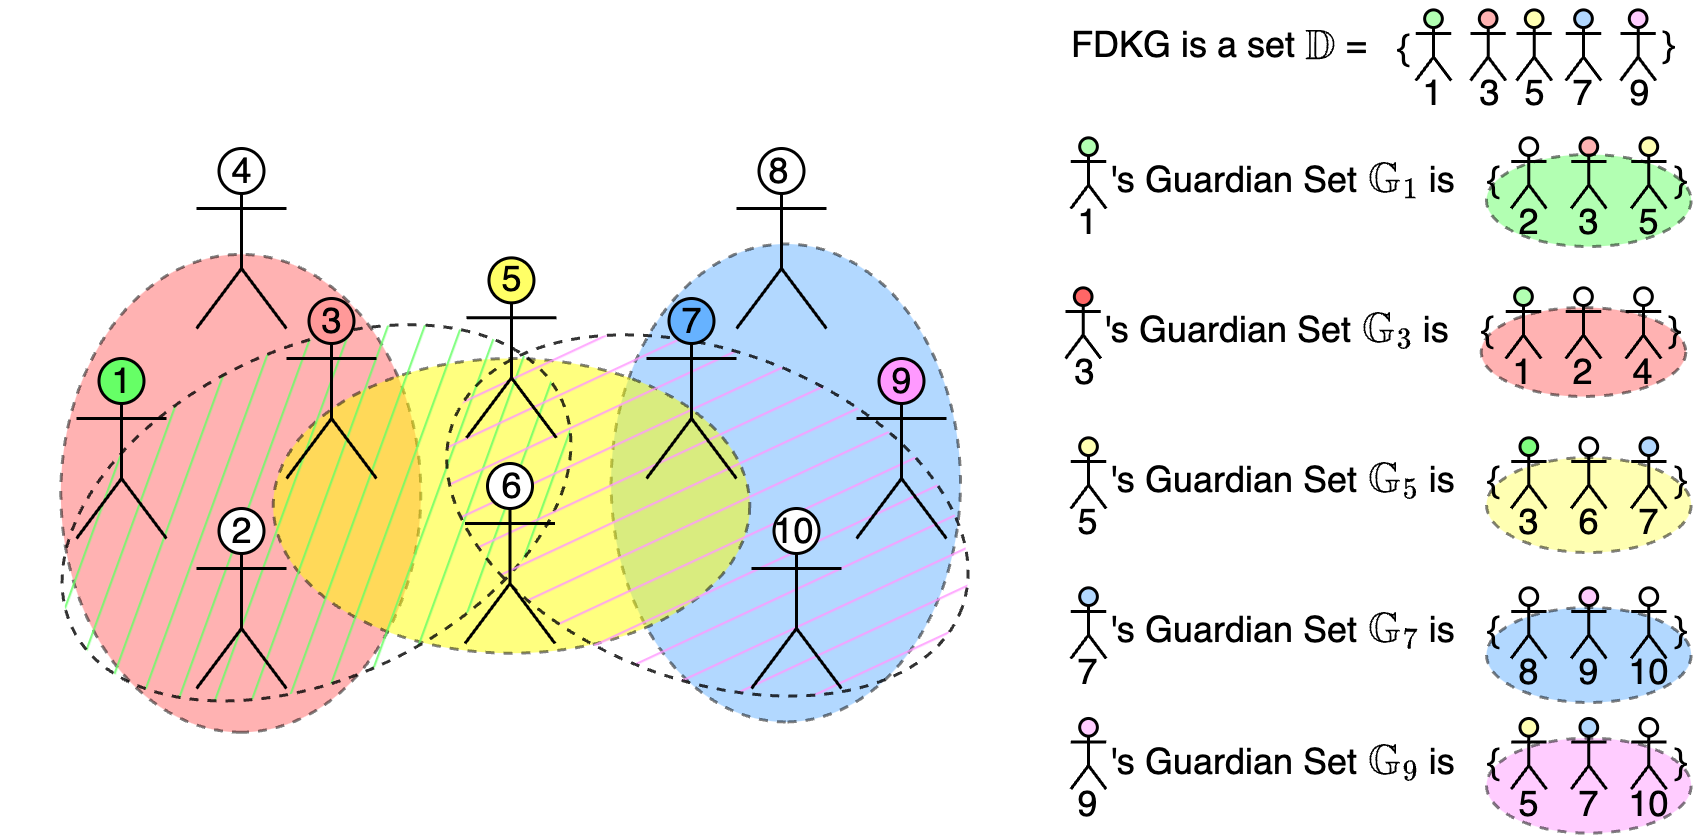
\includegraphics[width=\textwidth]{FDKG.png}
    \caption{Federated Distributed Key Generation}
    \label{fig:FDKG}
\end{figure}

The process for each participating party is as follows:

\begin{enumerate}
    \item \textbf{Party $P_1$}:
    \begin{itemize}
        \item Chooses Guardian Set $\mathbb{G}_1 = \{P_2, P_3, P_6\}$.
        \item Samples a random polynomial $f_1(X) \in_R \mathbb{Z}_q[X]$, and computes decryption key $d_1 = f_1(0)$.
        \item Splits $d_1$ among $\mathbb{G}_1$, resulting in shares $\PartialDecryptionKeyShare{1}{2}, \PartialDecryptionKeyShare{1}{3}, \PartialDecryptionKeyShare{1}{6}$.
    \end{itemize}

    \item \textbf{Party $P_4$}:
    \begin{itemize}
        \item Guardian Set \GuardianSetOf{4} = $\{P_3, P_5, P_6\}$.
        \item Samples random polynomial $f_4(X)$, and computes decryption key $d_4$
        \item Splits $d_4$ among $\mathbb{G}_4$, resulting in shares $\PartialDecryptionKeyShare{4}{3}, \PartialDecryptionKeyShare{4}{5}, \PartialDecryptionKeyShare{4}{6}$.
    \end{itemize}

    \item \textbf{Party $P_8$}:
    \begin{itemize}
        \item Guardian Set \GuardianSetOf{8} = $\{P_5, P_6, P_7\}$.
        \item Samples random polynomial $f_8(X)$, and computes decryption key \IthDecryptionKey{8}.
        \item Splits \IthDecryptionKey{8} among \GuardianSetOf{8}, resulting in shares $\PartialDecryptionKeyShare{8}{5}, \PartialDecryptionKeyShare{8}{6}, \PartialDecryptionKeyShare{8}{7}$.
    \end{itemize}

    \item \textbf{Party $P_{10}$}:
    \begin{itemize}
        \item Guardian Set \GuardianSetOf{10} = $\{P_7, P_8, P_9\}$.
        \item Samples random polynomial $f_{10}(X)$, and computes decryption key \IthDecryptionKey{10}.
        \item Splits \IthDecryptionKey{10} among \GuardianSetOf{10}, resulting in shares $\PartialDecryptionKeyShare{10}{7}, \PartialDecryptionKeyShare{10}{8}, \PartialDecryptionKeyShare{10}{9}$.
        
    \end{itemize}
\end{enumerate}

\subsection*{Conclusion of the FDKG Example}

In this FDKG scenario, we identified a minimal set of parties \(\{P_3, P_5, P_6, P_7, P_8\}\) that guarantees Decipherability (as defined in Definition \ref{def:decipherability}) and minimal sets \(\{P_3, P_5\}\) and \(\{P_6, P_7\}\) that can induce a Lock-in state (as defined in Definition \ref{def:lock-in}).

\paragraph{Decipherability}
The set \(\{P_3, P_5, P_6, P_7, P_8\}\) ensures Decipherability as it contains at least two members from each guardian set, thereby meeting the \(t\)-out-of-\(k\) requirement for share publication. Specifically, \(\{P_3, P_6\}\) satisfies \(\mathbb{G}_1\) and \(\mathbb{G}_4\); \(\{P_5, P_6\}\) satisfies \(\mathbb{G}_8\); and \(\{P_7, P_8\}\) satisfies \(\mathbb{G}_{10}\).

\paragraph{Lock-in}
1. For \(\{P_3, P_5\}\), if these parties do not participate, \(\mathbb{G}_1\) and \(\mathbb{G}_4\) lack sufficient shares due to the absence of \(P_3\), and \(\mathbb{G}_4\) and \(\mathbb{G}_8\) lack sufficient shares due to the absence of \(P_5\), leading to a Lock-in.
2. For \(\{P_6, P_7\}\), the absence of \(P_6\) affects \(\mathbb{G}_1\), \(\mathbb{G}_4\), and \(\mathbb{G}_8\), while \(P_7\)'s absence affects \(\mathbb{G}_8\) and \(\mathbb{G}_{10}\), also leading to a Lock-in.

\paragraph{Privacy}
Privacy in the FDKG system is compromised when all parties from a Decipherability set are malicious. For example, if \(\{P_3, P_5, P_6, P_7, P_8\}\) colludes they can collectively reconstruct the secret \DecryptionKey.

\section{System Implementation}

\subsection{Consensus and Networking}

\begin{figure}
    \centering
    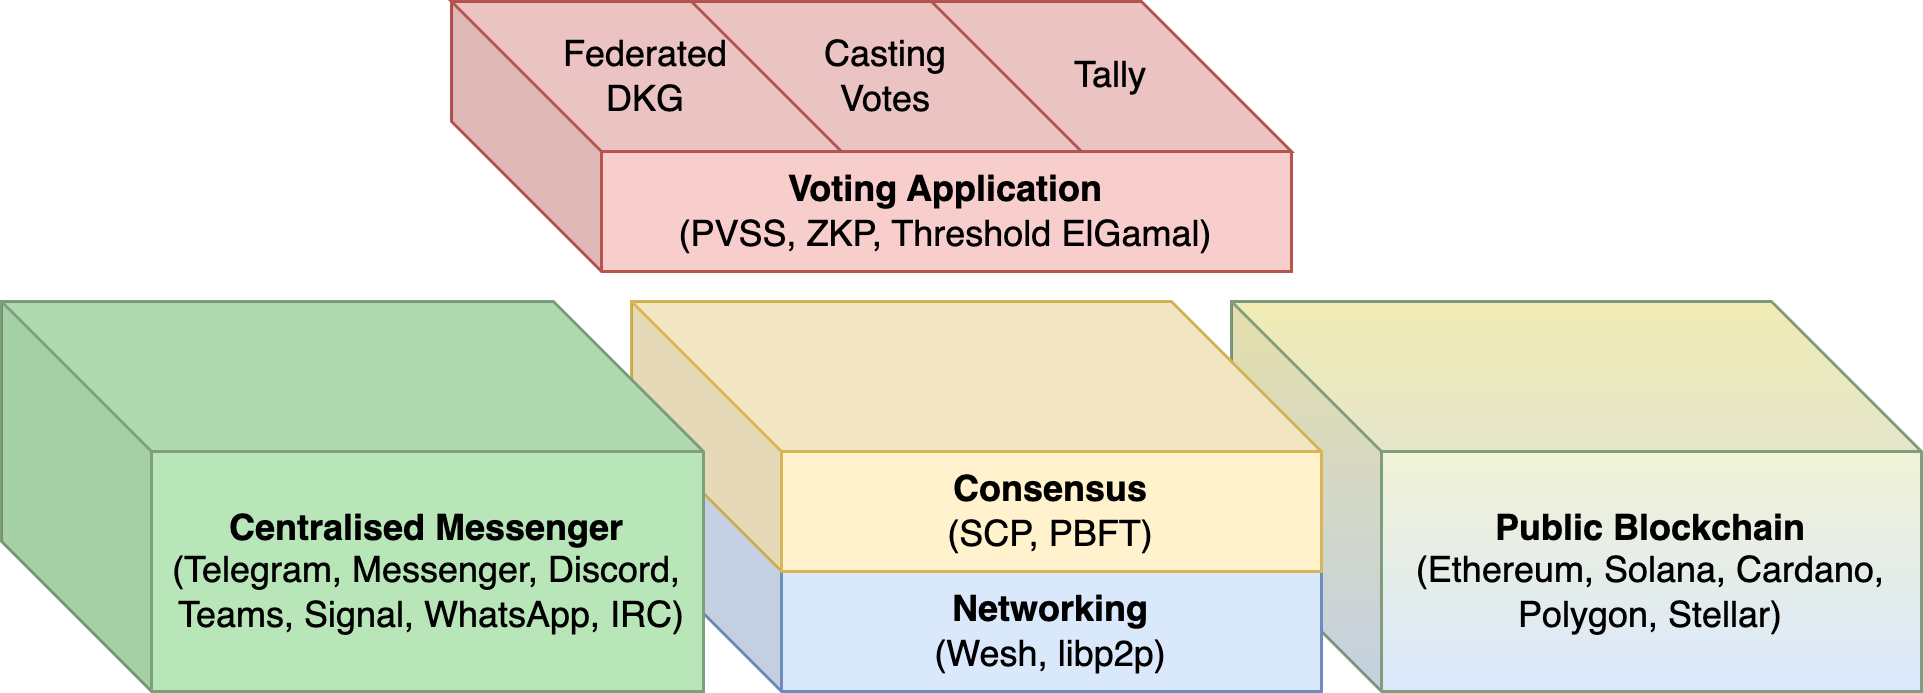
\includegraphics[width=\textwidth]{stack-bc.png}
    \label{fig:stack-bc}
    \caption{System architecture.}
\end{figure}

\begin{itemize}
    \item Ad-hoc blockchain network
    \item p2p networking via async mesh network https://wesh.network/
    \item FBA or Tendermint
    \item Or, a public blockchain with ERC4337 paymaster to cover the transaction costs
\end{itemize}

\section{Experimental Results}

\begin{table}
\centering
\label{table:plonk-time}
\caption{Execution time of the PLONK prover in seconds.}
\begin{tabular}{|c|c|c|c|c|}
    \hline
    \multicolumn{5}{|c|}{PLONK} \\
    \hline
    \multicolumn{3}{|c|}{\textrm{PROOF}_\textrm{FDKG}} & \multirow{2}{*}{\textrm{PROOF}_\textrm{BALLOT}} & \multirow{2}{*}{\textrm{PROOF}_\textrm{PD}} \\
    \cline{1-3}
    1 of 2 & 2 of 3 & 3 of 4 & & \\
    \hline
    67.753s & 71.902s & 146.026s & 16.822s & 8.602s/share\\
    \hline
\end{tabular}
\end{table}

\begin{table}
\centering
\label{table:groth16-time}
\caption{Execution time of the Groth16 prover in seconds.}
\begin{tabular}{|c|c|c|c|c|}
    \hline
    \multicolumn{5}{|c|}{Groth16} \\
    \hline
    \multicolumn{3}{|c|}{\textrm{PROOF}_\textrm{FDKG}} & \multirow{2}{*}{\textrm{PROOF}_\textrm{BALLOT}} & \multirow{2}{*}{\textrm{PROOF}_\textrm{PD}} \\
    \cline{1-3}
    1 of 2 & 2 of 3 & 3 of 4 & & \\
    \hline
    1.388s & 2.135s & 2.414s & 0.747s & 0.506s/share\\
    \hline
\end{tabular}
\end{table}

\begin{table}
\centering
\label{table:groth16-size}
\caption{Message size for each phase using Groth16 proving system.}
\begin{tabular}{|c|c|c|c|c|}
    \hline
    \multicolumn{5}{|c|}{Groth16} \\
    \hline
    \multicolumn{3}{|c|}{\textrm{PROOF}_\textrm{FDKG}} & \multirow{2}{*}{\textrm{PROOF}_\textrm{BALLOT}} & \multirow{2}{*}{\textrm{PROOF}_\textrm{PD}} \\
    \cline{1-3}
    1 of 2 & 2 of 3 & 3 of 4 & & \\
    \hline
    6.476 KB& 8.928 KB & 11.412 KB & 2.310 KB & 2.548 KB/share\\
    \hline
\end{tabular}
\end{table}

\begin{table}
\centering
\label{table:plonk-size}
\caption{Message size for each phase using Plonk proving system.}
\begin{tabular}{|c|c|c|c|c|}
    \hline
    \multicolumn{5}{|c|}{Plonk} \\
    \hline
    \multicolumn{3}{|c|}{\textrm{PROOF}_\textrm{FDKG}} & \multirow{2}{*}{\textrm{PROOF}_\textrm{BALLOT}} & \multirow{2}{*}{\textrm{PROOF}_\textrm{PD}} \\
    \cline{1-3}
    1 of 2 & 2 of 3 & 3 of 4 & & \\
    \hline
    7.825 KB& 10.332 KB & 12.817 KB & 3.671 KB & 3.920 KB/share\\
    \hline
\end{tabular}
\end{table}

\begin{figure}
    \centering
    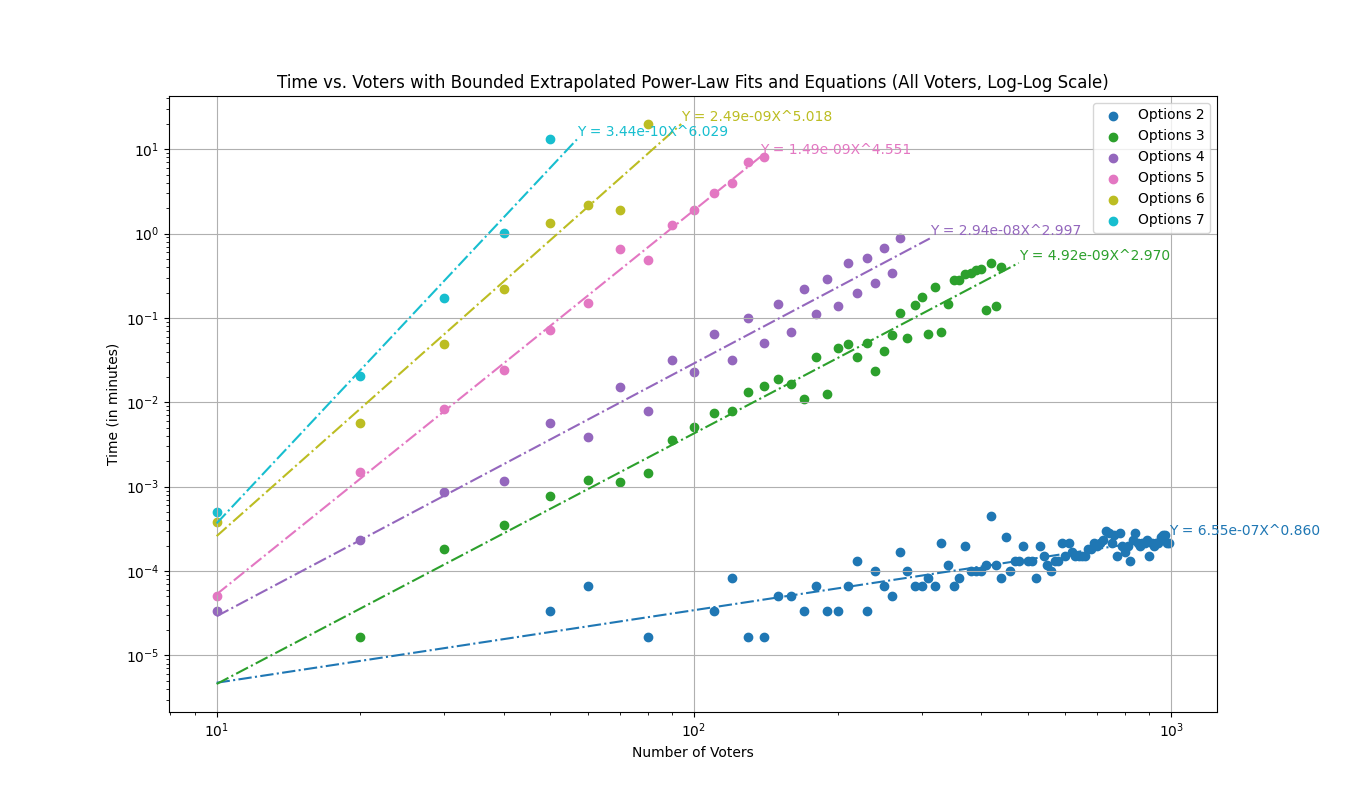
\includegraphics[width=\textwidth]{dlog-search-time.png}
    \caption{Time required to solve DLP with respect to number of candidates and number of voters.}
    \label{fig:dlog-search}
\end{figure}
Finally the offline tally requires extracting number of voters for each party. To do so we have to solve the Discrete Logarithm Problem (DLP) for the final output point $M = H * \sum_i v_i$. The goal is to find the scalar value $\sum_i v_i$ which when multiplied by $H$ gives the voting output $M$. In general the problem of solving DLog is considered infeasible and so the security of DLog-based crypto systems holds. However, for small number of voters the problem can be solved using exhaustive search within a reasonable time. To extract each $x_i$ we use the technique described in~\cite{haoAnonymousVotingTworound2010}. Figure~\ref{fig:dlog-search} shows the time required to solve DLP.

Analysis of the measurements shows that time required to find the DLog follows the power-law $Y=aX^b$ where parameter $b$ is linear with the number of options, which is an expected behaviour.


%TODO: 
\section{Discussion}

\section{Conclusion and Future Work}

We find two possible paths of optimisations. First is in optimising the proof time and size by batching proofs together. 
The second one is on implementing the solution on-chain but making it gasless with the use of paymaster introduced in ERC-4337, making the votes gasless.

\section{Acknowledgments}


\bibliographystyle{IEEEtran}
\bibliography{bibliography}

\end{document}